The design of the \CaF{} chip experiment was motivated by three main factors:
the need to integrate with the existing experiment, the core proposal of
confining molecules close to a microwave guide, and the practicalities of
fabricating the chip. In this chapter I will describe how the first two factors
informed the design choices, with changes due to fabrication discussed in
chapter~\ref{fab}. The design will be further justified by simulation in
chapter~\ref{sim}.
%
We begin with a discussion of the existing experiment. I will then give an
overview and motivation of the design of the new experiment.


\section{Existing \CaF{} experiment}

In this section I will present a summary of the process used to produce
ultracold \CaF{} molecules in a magnetic trap, which we intend to load onto the
chip trap. We will consider the various stages of the process, which is
presented in \myfigref{overview:fig:CaFcartoon}. First a beam of \CaF{}
molecules is created using a buffer gas
source~\cite{Truppe2018}. The beam is then slowed by
application of slowing light opposing its direction of
travel~\cite{Truppe2017a}. The slowing light can also be applied in the
transverse direction to reduce the broadening of the beam during its flight.
The molecules are captured in a MOT~\cite{Williams2017} and cooled in optical
molasses~\cite{Truppe2017} before being optically pumped into a weak field
seeking state~\cite{WilliamsMagnetic2018}. This allows for magnetic trapping
and transport of the molecules.

\begin{figure}
  \centering
  \includegraphics{figs/overview/cartoon.pdf}
  \caption{A schematic of the \CaF{} source, slowing region and MOT chamber.
  \CaF{} molecules (grey cone) are produced by the buffer gas cell, and are
  slowed by longitudinal slowing and transverse cooling light (green,
  \pewpew{S}{00}). The molecules are then captured in a MOT (MOT light
  \pewpew{}{00} and repumps combined are shown here in orange) where
  they can be further cooled and transferred to a magnetic trap. The molecules
  can then be transported out of the chamber by the MTT in the direction of the
  pink arrow. A detailed view of the source is shown in
  \myfigref{overview:fig:source}}
  \label{overview:fig:CaFcartoon}
\end{figure}

This section is merely an outline of a very broad topic, but one that is
essential to the context of the chip. A more complete description  can be found
in \inlineref{Jurgilas2021}.

\subsection*{\CaF{} energy structure and constants}

The energy structure of \CaF{} is depicted in
\myfigref{overview:fig:CaFenergy}. Here we show only the levels that are
pertinent to this thesis, those being the X, A and B electronic levels up to
vibrational level $v= 3, 2 \text{and} 0$ respectively.  For the X state, we
will discuss both the $N=0\text{and}1$ states.
Figure~\ref{overview:fig:CaFenergy} and \mytableref{overview:table:lasers} also
label the various lasers that are used to addressed the \CaF{} transitions. We
label these as \pewpew{}{vv'} where $v$ ($v'$) is the lower (excited)
vibrational level that the laser addresses. The superscript $S$ is used to
distinguish the $X\rightarrow B$ transition.

\begin{figure}
  \centering
  \includegraphics[width=0.8\textwidth]{figs/energylevels/main_sbs.pdf}
  \caption{
    The energy levels of \CaF{} are shown, along with the lasers that will be
    used to address the various transitions (further information is found in
    \mytableref{overview:table:lasers}). The branching ratios for the allowed
    decays are shown with dashed lines. Note that the $X(N=0)$ level is
    included, but for simplicity the $X(N=2)$ level is omitted. The box shows
    the hyperfine levels of $X(N=1, v=0)$. This figure is adapted from
    \inlineref{Williams2018}. 
  }
  \label{overview:fig:CaFenergy}
\end{figure}

\begin{table}
  \centering
\begin{tabular}{llll}
  Symbol & Ground state & excited state & wavelength (\si{\nano\meter}) \\
  \pewpew{}{00} & $X(v=0)$ & $A(v=0)$ &  606 \\
  \pewpew{S}{00} & $X(v=0)$ & $B(v=0)$ & 531 \\
  \pewpew{}{01} & $X(v=0)$ & $A(v=1)$ & 628 \\
  \pewpew{}{12} & $X(v=1)$ & $A(v=2)$ & 628 \\
  \pewpew{}{23} & $X(v=2)$ & $A(v=3)$ & 628 \\
  \pewpew{}{10} & $X(v=1)$ & $A(v=0)$ & 585 \\
 \hline
\end{tabular}
\caption{
  The various laser transitions used in this thesis are tabulated.
  \pewpew{}{10} is included for completion, and will be explained in
  chapter~\ref{experiment}.
  }
  \label{overview:table:lasers}
\end{table}

Also shown by the dashed lines are the permitted decay paths, along with their
branching ratios. One of the reasons \CaF{} is chosen for study over other
molecules is its highly diagonal Franck-Condon factors, so that most decays
occurr with $v'=v$. However for large numbers of scattered photons we must
employ the various repump lasers to avoid pumping into states that are dark to
the cooling light, as we shall see when we discuss slowing of the beam and the
MOT.

Hyperfine splitting occurs in \CaF{} due to the spin-half contribution of the
fluorine atom. This is not resolved in the $A$ state, but must be accounted for
in the $X$ state. The hyperfine splitting is shown in the box of
\myfigref{overview:fig:CaFenergy}. In the $B$ level, the $F=0$ and $F=1$ states
are split by \SI{20}{\mega\hertz}, which can be neglected for the purposes of
our discussion. A full description of the \CaF{} energy structure and various
constants can be found in \inlineref{Anderegg2019a}, those that are most useful
are presented in \mytableref{overview:table:constants}.

\begin{table}
  \centering
\begin{tabular}{lll}
  Constant & Symbol & Value \\
  Mass & m & \\
  % TODO I think Mike gave this to me, but it it for particular transitions?
  Electric dipole moment & $\mu_e$ & \\
  Magnetic dipole moment & $\mu$ & \\
 \hline
\end{tabular}
\caption{
  Various constants for \CaF{} taken from \inlineref{Anderegg2019a}.
  % TODO Also taken from elsewhere?
  }
  \label{overview:table:lasers}
\end{table}

\subsection*{Buffer gas source}

We begin all our experiments by creating a pulsed beam of \CaF{} molecules
using a buffer gas source. Such a device operates by using a buffer gas (in
this case helium) to thermalise between a cold cell and warm molecules. The
molecules then exit through an aperture to form a beam. The \CaF{} molecules are also
created inside the beam from \SFsix{} gas and calcium atoms, which are ablated
from a target by a high-power Nd:YAG laser.

The buffer gas cell is pictured in \myfigref{overview:fig:source}. A \Ca{}
target is positioned inside the cell, opposite an aperture for optical access
with the ablation laser. This is mounted on a rotating stage, so that when one
region is depleted another can be targeted. We flow \SFsix{} into the cell at
\SI{270}{\kelvin}, which reacts with ablated \Ca{} atoms to form \CaF{}. The
cell is cryogenically cooled to \SI{4}{\kelvin} and is designed to optimise the
flow of \He{} so as to thermalise with \CaF{} and guide it to the exit aperture
without the creation of vortices, where the molecules can be
trapped~\cite{Truppe2018}. For this reason \He{} enters the back of the cell at
\SI{4}{\kelvin} and flows towards the exit aperture.

\begin{figure}
  \centering
  \cm{TODO Cell figure}
  \caption{}
  \label{overview:fig:source}
\end{figure}

\cm{For charcoal, cite Sarunas' ref 121}
In order to remove excess helium, a copper shield, coated with coconut charcoal
and also cooled to \SI{4}{\kelvin} is used as a helium absorber. These are
theramlly cycled overnight when the source is not in use to avoid saturation.
A mechanical shutter is also installed after the cell to minimise any increase
in background pressure due to \He{} gas leaving the source.

As noted in \inlineref{Jurgilas2021}, this buffer gas source originally
produced up to \SI{5E10}{molecules/steradian} molecules in $X(N=1, v=0)$ with a
mean velocity of \SI{160}{\meter\per\second}~\cite{Truppe2018} but its
performance has degraded since this original report, and we now capture only
\SIrange{50}{60}{\percent} lower capture in the MOT than we have previously
observed.

\subsection*{Slowing the beam}

The buffer gas source produces a beam of molecules with slower average velocity
than, for example, a \cm{supersonic source} but they are still far above the
capture velocity of our MOT. The beam's velocity can be further reduced by
radiation pressure due to a counter-propagating beam of \pewpew{S}{00}
slowing light. This is chirpped to account for the change in Doppler shift of the transition
frequency as the molecules slow. The slowing light is also combined with the
\pewpew{}{10} repump light to avoid pumping into the $X(v=1)$ state. To again
account for Doppler shift during slowing, the repump light is frequency
broadened by \SI{300}{\mega\hertz}.

We apply the light for \cm{time}, which slows over approximately
\SI{90}{\centi\meter} of travel from the buffer gas cell's exit aperture.
Linear chirps used in previous experiments have shown to reduce the velocity to
\cm{??}, however an exponential chirp proposed \cm{by Harvard} and implemented
\cm{by Sarunas} produced a \SIrange{60}{80}{\percent} improvement in the number
of molecules in the MOT.

Slowing the beam has the undesirable effect of increasing the transverse
velocity of the molecules. This is due to the random walk of the molecules as
they scatter photons from the slowing light. One method of reducing this effect
is to focus the combined light so as to converge towards the cell to reduce
transverse scattering. 

\subsection*{Transverse cooling}

\cm{It's not chirped, we use sidebands -- intoduce \pewpew{T}{00}}

The transverse heating effect can be further reduced by applying
slowing beams in the transverse direction, also on the $\mathcal{L}_{00}^S$
transition. The slowing procedure described above is carried out
simultaneously, providing the remixing of dark ground states and the $v=1$
repump light.
%
Scattering of light in the transverse direction can collimate the beam, and has
been shown to improve the population of the MOT by a factor of $\sim3$. 

\subsection*{Capture in a MOT}

Positioned \cm{\SI{130}{\centi\meter}} from the cell's exit aperture is the 
centre of the MOT chamber. The MOT magnetic field is provided by in-vacuum
anti-Helmholtz coils, and the \pewpew{}{00}, \pewpew{}{10}, \pewpew{}{21},
\pewpew{}{32} light is incident on the molecules in combined beams entering
on all three axes and retroreflected to provide restoring beams in both
directions (see \myfigref{overview:fig:cartoon}).
%
The operating principle of the \CaF{} MOT is similar to those described in
\cm{ref section in theory}, but with some key differences that we outline
here. A complete description is far beyond the scope of this overview, and has
been described in detail elsewhere, for example see \cm{Hannah's thesis,
  Sarunas' thesis, something else not a thesis?}

First, the significant number of photon scatters \cm{what is it?} in the MOT
mean that it is necessary to apply the vibrational repumps (\pewpew{}{10},
\pewpew{}{21} and \pewpew{32}) along with the main cooling light
(\pewpew{}{00}), or else molecules will be pumped into these dark states. All
of these beams must be \cm{equipped} with the r.f.\ sidebands to address the
hyperfine levels of the $X$ state (recall that the hyperfine levels of $A$ are
unresolved).

The second nuance is that the \CaF{} MOT is that it is a type-II MOT~\cite{},
meaning that the angular momentum of the excited state ($A(v=0)$, with $F'=1$)
is less than that of the ground state ($X(v=0)$ with $F=2$). Unlike a type-I
MOT (where $F'>F$), it is therefore possible for a molecule that has been
pumped into the excited state to decay into a dark state, or into a state that
is anti-trapped by the MOT~\cite{}.
%
To resolve this, we employ a dual-frequency MOT. The main MOT transition is
addressed by the \pewpew{}{00} light, with r.f.\ sidebands added to address the
different hyperfine levels. The sideband addressing the $F=1$ hyperfine state
is given opposite polarisation, and simultaneously serves as a second frequency
for the $F=2$ state. This ensures that the normally anti-trapped states are
repumped by the restoring beam into the MOT cycle. The $F=2$ level is now
strongly trapped and although the other levels remain weakly trapped, this is
sufficient to create a strong MOT.

A simplified case with $F=0$ and $F'=1$ is shown in
\myfigref{overview:fig:dualfreq}. When there is no blue-detuned light, any
molecule that decays into the $m_F=-1$ state can be lost from the cycle. When
the blue-detuned light is present these molecules can be repumped. Since this
transition has a change in $m_F$ of $\Delta m_F = m'_F- m_F=1$, we require the
blue-detuned light to have $\sigma_+$ polarisation.

\begin{figure}
  \centering
  \cm{TODO: remake Hannah's fig 4.1 (RHS only)}
  \caption{
    A dual frequency scheme for the type-II case $F'=0$, $F=1$. The molecules
    in each state (circles) can be pumped by their corresponding red- (blue-)
    detuned light. This figure is adapted from one in \inlineref{Williams2018}.
  }
  \label{overview:fig:dualfreq}
\end{figure}

The capture velocity of the MOT is \cm{??} meaning that we are typically able
to capture $??$ molecules from our beam. The MOT population can be estimated by
looking at the scatter, or by turning off the light and performing
light-induced fluorescence imaging using \pewpew{}{00}. The MOT temperature is
typically \cm{}, and this can be further reduced by lowering the intensity of
\pewpew{C}{00}~\cite{Truppe2017} \cm{what is final temp?}

\subsection*{Optical molasses}

Sub-Doppler cooling of \CaF{} is achievable by employing a blue-detuned
molasses. In this scheme the MOT coils are switched off, and \pewpew{C}{00}
is detuned to be blue-detuned \cm{by how much?}.  Consider the example of a
$F=1$ hyperfine level ground state, and $F=0$ excited state which is shown in
\cm{fig like Hannah's 5.1}. A polarisation gradient is established across the
molasses. In regions where the polarisation is $\sigma_-$ ($\sigma_-$) only the
$m=1$ ($m=-1$) ground state is coupled to the light.

The a.c.\ Stark shift now acts on the bright states, meaning that as they move
through the light field they lose kinetic energy. Near the peak of the energy
shift, the bright state molecules are preferentially pumped into the dark
state. Meanwhile the dark states will adiabatically transfer back to bright
states, which occurs preferentially at regions where the bright and dark states
are close in energy. This cycle then repeats, resulting in the molecule losing
energy as it passes through the light field.

% TODO Cite Molecules cooled belowo DOppler limit and
% Weidemu ̈ller, M., Esslinger, T., Ol’shanii, M. A., Hem- merich, A. & Ha ̈nsch, T. W. A novel scheme for efficient cooling below the photon recoil limit. EPL 27, 109–114 (1994).

In the \CaF{} experiment, the situation is not so simple. We must account for
intensity gradients as well as those of polarisation, and of course the real
experiment occurs in three dimensions not one. Details of this scheme can be
found in \inlineref{1367-2630-18-12-123017} and~\cite{Truppe2017}.

\subsection*{Magnetic trapping and transport}

\cm{inc. optical pumping}

At this stage we also introduce three stretched states in \CaF{}. These states
lie in the $X$ electronic level, and are denoted $\ket{N}_\text{str} = \ket{N,
m_N}_\text{rot}\ket{S, m_S=S}\ket{I,m_I=I}$, where the degeneracy must be
lifted by the application of an external magnetic field, $m_X$ is then the
projection of $X$ onto this field's axis. The stretched states are of interest
because they are not only weak-field seekers, but the transitions between
neighbouring stretched states
($\ket{N}_\text{str}\leftrightarrow\ket{N+1}_\text{str}$) are highly
insensitive to magnetic fields.


\subsection*{Other experiments}
% TODO Is this section really necessary?

% TODO Rework this para? Maybe it just becomes a sentence, something like "we
% use this setup for lots of things, not we want to use it for chip instead"
The \CaF{} MOT is the workhorse of our experiment, providing molecules which
can be further cooled cooled further (as discussed above) used for experiments
in collisions with \Rb{} atoms (see \inlinerefs{Jurgilas2021, JurgilasIOP2021,
PhysRevLett.126.153401}) and optical tweezers. The tweezer experiment is
undertaken in the neighbouring tweezer chamber, which is loaded by transporting
molecules in a magnetic transport trap (MTT), a quadrupole trap with coils
mounted on a transport stage outside the vacuum chamber. This transport of the
molecules is similar to that used in
\inlinerefs{Lewandowski2003,PhysRevResearch.1.033035} and elsewhere, it will be
discussed further below and in \cm{transport chapter}.


\section{Design requirements and overview}

%\begin{itemize}
%  \item Andr\'e proposal, want to strongly couple to coplanar waveguides
%  \item Want to do quantum operations with rotational stretched states
%  \item Need small size scale
%  \item Height limited by VdW force, as per Ed's notebook (Charles Smith also said something
%    about charges causing decoherence?) height gives scale size
%  \item We want to use magnetic trapping rather than electric (as explained
%    in QSUM report: long coherence times and easier to load (?))
%  \item Need to be able to load (one step is no good, ref. next chapter)
%\end{itemize}

As discussed in \cm{the introduction} the aim of this project is ultimately to
trap molecules in close proximity to microwave resonators so that we can
perform coherent control of quantum states on the rotational transitions in the
molecules.
%
Following the proposal by \inlineref{Andre2006}, this can be achieved in a chip
architecture, with the molecule trapped as close to the resonator as possible.
%
\cm{Calculation of VdW force to get the 10um figure}
%
Given that the molecules will be $\sim\SI{10}{\micro\meter}$ from the surface,
we will require that trapping electronics will be on a smaller scale than this
so that trapping potential is \cm{sufficiently localised}.  Features of such a
size can be easily created by standard photolithography techniques.

Additionally, we aim to integrate the chip trap into our existing \CaF{}
experiment. This can be done by the addition of a new chamber to our setup,
shown in \myfigref{overview:fig:vacuumsystem}. The chip chamber will be
positioned along the existing MTT axis, allowing extension of the transport
system and the delivery of molecules to this chamber. \CaF{} molecules can then
be transferred onto the chip trap.

\begin{figure}[htb]
  \centering
  %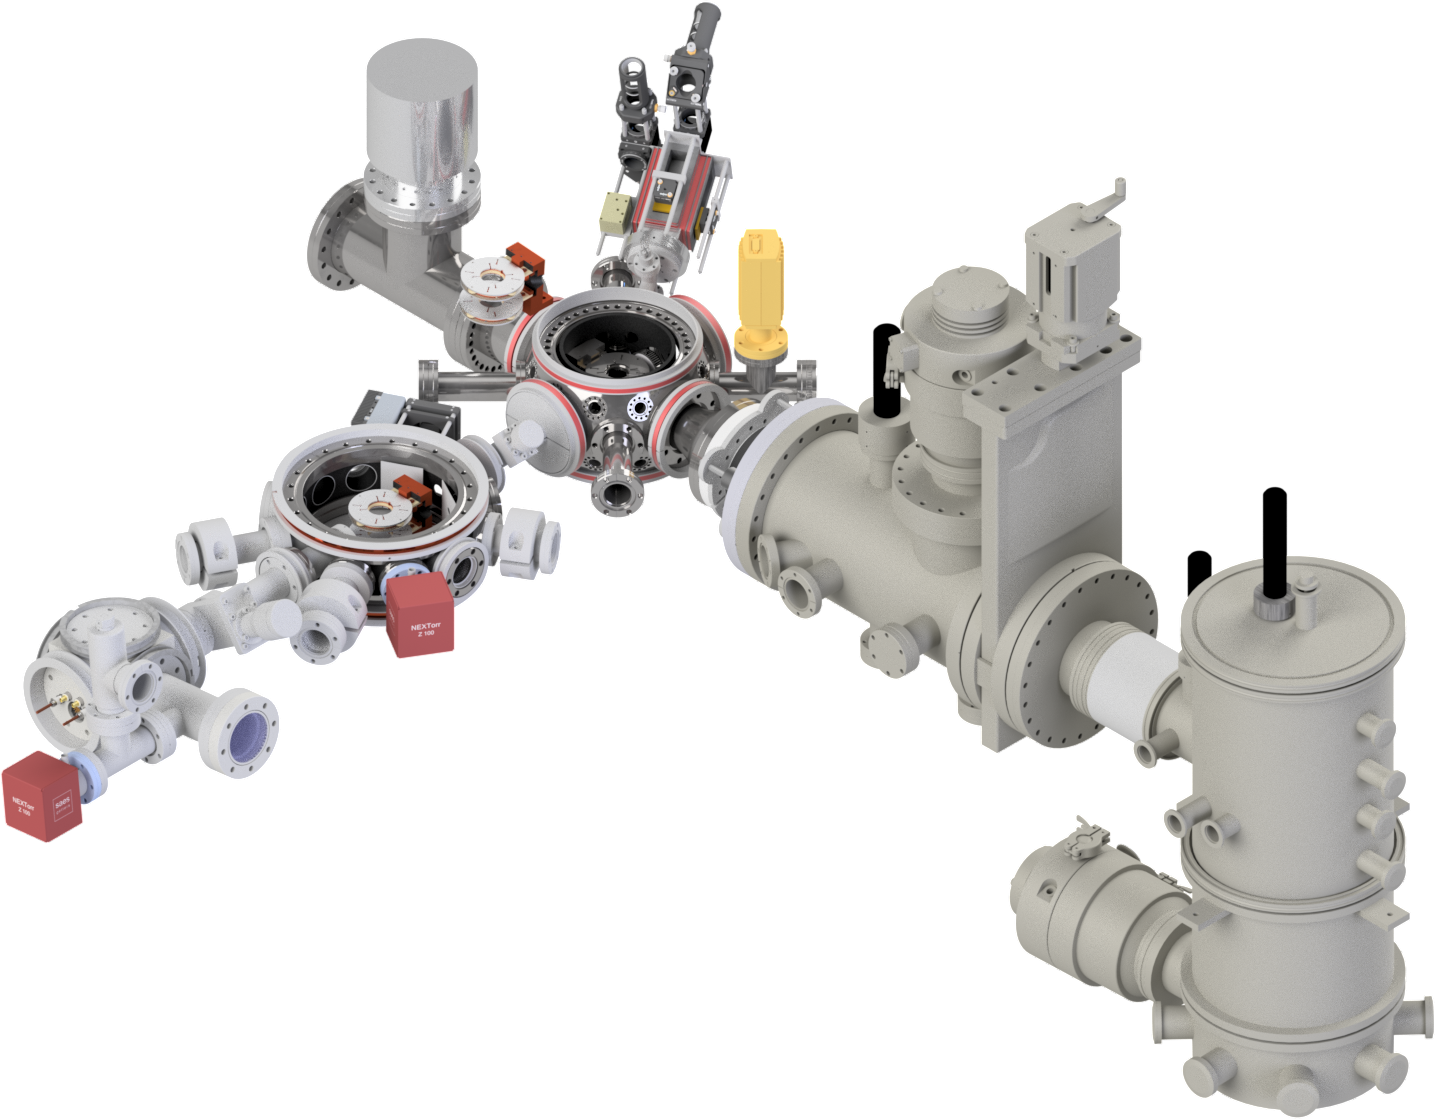
\includegraphics[width=0.7\textwidth]{figs/overview/apparatus_04_crp.png}
    \begin{tikzpicture}
      \node[anchor=south west,inner sep=0] (image)
{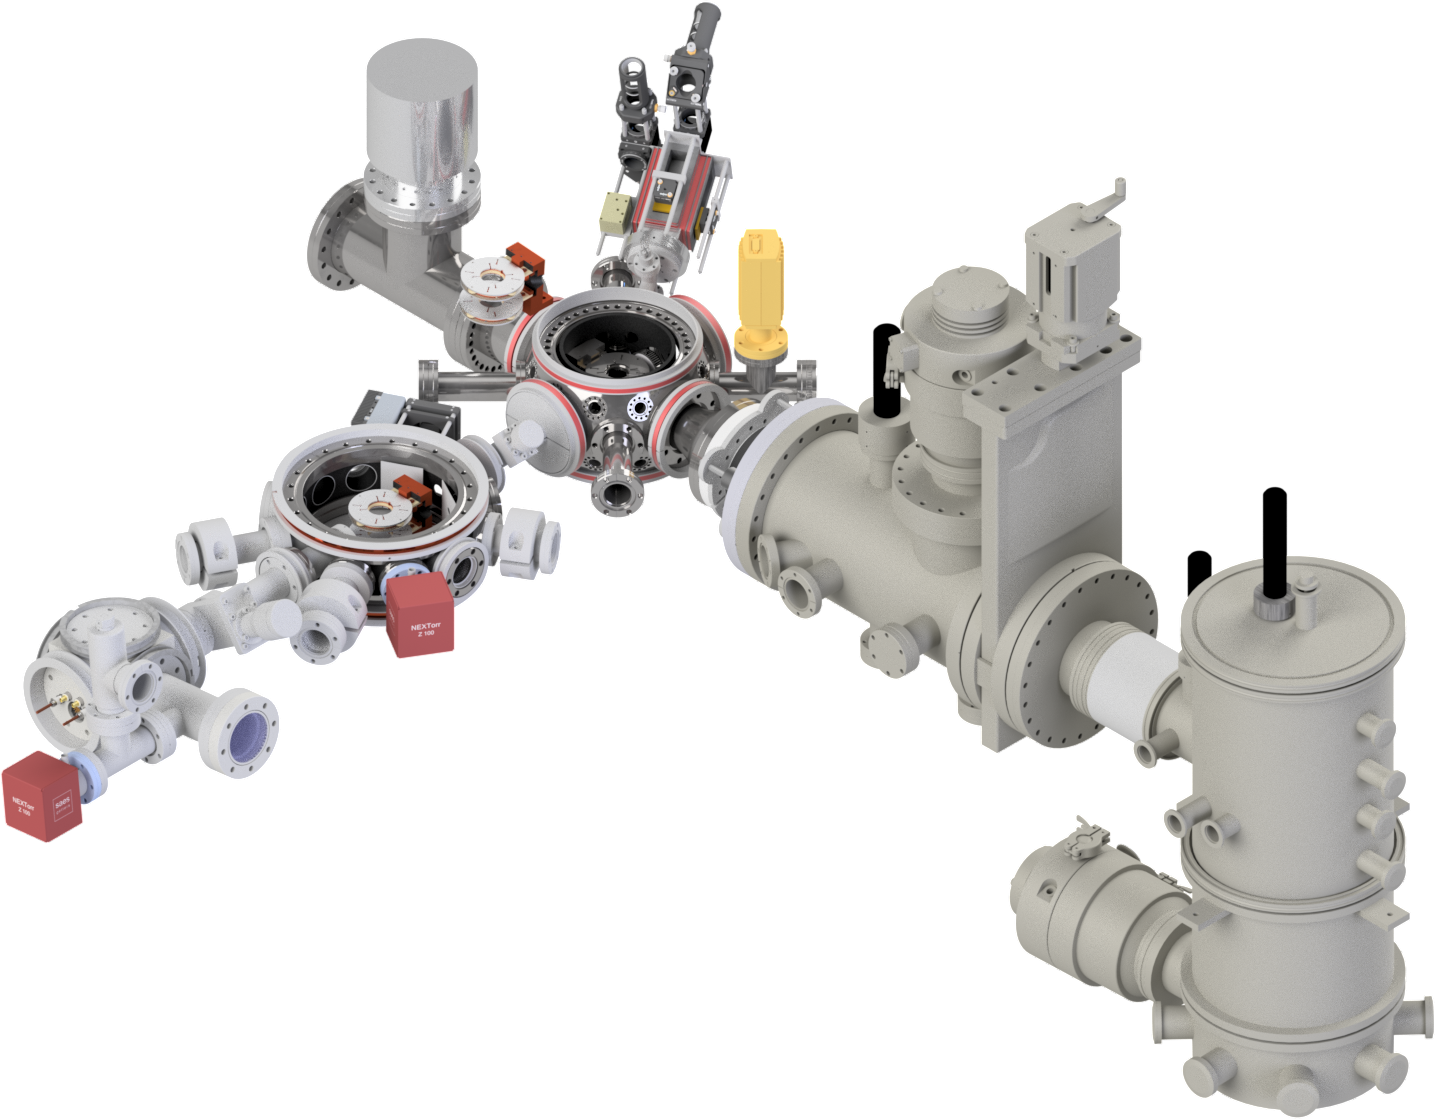
\includegraphics[width=0.8\textwidth]{figs/overview/apparatus_04_crp.png} };
      \begin{scope}[x={(image.south east)},y={(image.north west)}]
        \draw [-stealth] (0.45, 0.35) -- (0.45,0.52);
        \node[] at (0.46,0.3) {\small MOT chamber};
        \draw [-stealth] (0.18,0.23) -- (0.1, 0.3);
        \node[] at (0.21,0.2) {\small Chip chamber};
        \draw [-stealth] (0.15, 0.7) -- (0.2,0.63);
        \node[] at (0.12,0.72) {\small Tweezer chamer};
        \draw [-stealth] (0.7, 0.95) -- (0.52,0.85);
        \node[] at (0.72,0.99) {\small \Rb{} cell};
        \draw [-stealth] (0.95, 0.85) -- (0.8,0.7);
        \node[] at (0.97,0.89) {\small Slowing region};
        \draw [-stealth] (0.6, 0.2) -- (0.7,0.2);
        \node[] at (0.54,0.2) {\small Source};
      \end{scope}
    \end{tikzpicture}
  \caption{
    The \CaF{} experiment is shown along with the planned additional chip
    chamber. Not shown: external transport coils and transverse cooling region.}
  \label{overview:fig:vacuumsystem}
\end{figure}

At this point we note that the rotational stretched states of \CaF{} have been
demonstrated to have exceptionally long lifetimes in a macroscopic magnetic
trap~\cite{WilliamsMagnetic2018}. For this reason it was decided that using
magnetic traps, such as those describedin \cm{section} would be
preferable to the electrostatic traps suggested in \inlineref{Andre2006}. We
are now faced with the question of how exactly we can load molecules from the
MTT into the microscopic chip trap.
%
Fortunately this problem has previously been addressed for atom chips. For
example in \inlineref{Ott2001} \cm{fix phrasing} have transferred \cm{from a
similar transport trap to ours?} into a chip trap, via a macroscopic U-trap
that is aligned with the chip. This makes it easier to align the MTT and the
chip trap. The molecules can then be transferred between the traps by ramping
of the trapping currents in the U-wire and coils.
%
Molecules can similarly be transferred onto and between traps on the chip by
ramping of the trapping currents~\cite{}. Such a procedure is
non-tirival, and is the main subject of chapter~\ref{sim}.

To ensure that molecules are loaded into the smallest trap efficiently, we
again follow the footsteps of atom chips, and have designed  a series of traps
of decreasing size~\cite{Reichel1999}. For magnetic traps, the width of the
wires should decrease, so that the molecules remain \cm{highly localised around
the trap centre} throughout loading. 
%
Each wire trap will begin trapping at one height before the bias field is
increased to bring the trap centre closer to the surface (as per
\myeqref{theory:eqn:height}). We choose the wires to be Z-traps so as to avoid
any losses by spin-flips, and so we label the stages $\mathrm{ZX_i}$ for
initial (higher) traps and $\mathrm{ZX_f}$ for the final (lower) trap, with
$\mathrm{ZX}$ corresponding to the wire labels in
\mytableref{overview:table:wires}. Bias fields for all traps are to be provided
by external Helmholtz coils.

Each Z-wire should be sufficiently large maintain the currents required to form
a trap at height $z$ below the trap, whilst having a width and height  $w, h
\ll z$ so that that the current is highly localised compared to the cloud size.
%
In the case of the first Z-wire, the molecules are still \SI{3}{\milli\meter}
away from the trapping wire. If we demand a trap depth of
$k_B\times\SI{1}{\milli\kelvin}$, then we will require a trapping current of
\SI{30}{\ampere} to form a trap of this depth.  We will discuss in
chapter~\ref{fab} that the maximum wire height that can reliably be fabricated
is \SI{5}{\micro\meter}, and we expect that the wires will be able to carry a
maximum current density of \SI{6E10}{\ampere\per\meter\squared}, as was found
for a similar chip design in \inlineref{Treutlein2008}. The Z-wire will
have a width $w=\SI{200}{\micro\meter}$. The currents and widths of other wires
are calculated similarly.
%
All wires have been designed to
carry twice the current that is required in the loading scheme, so that there
is sufficient headroom for further experiments, and to reduce risk of
accidental damage to the chip during normal operation.
%
The axial length of the wires also decreases to gradually reduce the size of
the trapped cloud in the $x$ direction.  

% TODO Maybe need more detail here
\begin{table}
  \centering
\begin{tabular}{lrrrrr}
  Name & Axis length (\si{\milli\meter}) & Width (\si{\micro\meter})& $I_\text{max}$ & Trap height (\si{\micro\meter}) \\
 \hline
  U & 16 & N/A& 100 & 3000\\
  $\mathrm{Z0}$ & 12 & 200& 60& $3000\rightarrow1000$ \\
  $\mathrm{Z1}$ &  6 & 20& 6& $1000\rightarrow100$ \\
  $\mathrm{Z2}$ &  2 & 2& 0.6& $100\rightarrow10$ \\
 \hline
\end{tabular}
  \caption{Details on the wire dimensions, maximum current, and desired
  trapping heights. The wire design is shown in
  \mysubfigref{overview:fig:chiplayout}. Note that the U-wire current is
  limited by vacuum feedthroughs and not by the maximum current calculated by
  the wire dimensions.  The maximum currents have been designed for use at only
  50\% of their potential maximum ($I_\text{max}$).
  }
  \label{overview:table:wires}
\end{table}

The final chip design was informed both by the requirements here, the
simulations presented in chapter~\ref{sim} and the restrictions due to the
fabrication process, which will be discussed in chater~\ref{fab}. We tried
various different designs, but the final one that was chosen is shown in
\cm{fig}. It features the wires as stipulated in
\mytableref{overview:table:wires}, fanouts for connection to macroscopic
\cm{current delivery} and various other features that will also be explained in
chater~\ref{fab}.

\begin{figure}[ht]
  \centering
    \begin{overpic}[abs, width=0.45\textwidth]{figs/chip_present4.pdf}
      \put(10, 160){\small (i)}
      \put(60, 160){\small(ii)}
      \put(175, 60){\small(iv)}
      \put(110, 137){\small(iii)}
      \put(70, 90){\small \SI{20}{\micro\meter}}
      \put(112, 93){\small\SI{10}{\micro\meter}}
      \put(8, 42){\small $\mathrm{Z_0}$}
      \put(8, 10){\small $\mathrm{Z_1}$}
      \put(8, 200){\small $\mathrm{Z_2}$}
    \end{overpic}
  \caption{
    A schematic of
    the chip features, with the scaling exaggerated for visibility. The three
    overlapping Z-wires are shown and labeled. The gaps between the wires are
    highlighted.
    %
    Toward the left (i) is the
    electroplating connection pad and various features used for
    characterisation (ii). On Z2 it is possible to see several small pads used
    as anchors, to secure the thin wire to the substrate.  The axis of the
    $\mathrm{Z1}$ wire is labeled for reference (iii) and the other wires are
    similar. All of the above features  will be discussed further in
    chapter~\ref{fab}. The crest of Imperial College London (iv) is also
    included.}
  \label{overview:fig:chiplayout}
\end{figure}

Notice that this design does not incorporate microwave guides. These are to be
installed on a second level, separated from the trapping wires by a thin
insulating layer, on which we can fabricate coplanar waveguides~\cite{1127105}.
This stage of the project has not yet been reached, but the planned fabrication
procedure for microwave guides is discussed in \cm{ref section} and their
operation is discussed in chapters~\ref{mws} and \ref{squeeze}.

\begin{figure}
  \centering
  \begin{subfigure}[b]{0.45\textwidth}
    \includegraphics[width=\textwidth]{figs/overview/chamber_xsecarrow.pdf}
    \caption{}
  \end{subfigure}
  \hspace{1cm}
  \begin{subfigure}[b]{0.45\textwidth}
    \includegraphics[width=\textwidth]{figs/chip_pic_crop.png}
    \caption{}
  \end{subfigure}
  \caption{
  A cross section of the chip chamber is shown in (a). The arrow shows how
  molecules will enter the chamber, brought in by the MTT.
  In (b) we have the chip assembly fully constructed, with a view of the
    aluminium-core PCB (subchip) for current delivery. The
    microwave feedthroughs remain disconnected.
  }
  \label{overview:fig:chipchamber}
\end{figure}

% TODO Put exploded view with details in the experiment chapter

To facilitate all of this, the internals of the chip chamber have been designed
as shown (in cross section) in \mysubfigref{overview:fig:chipchamber}{a}.
Molecules can be brought in along the transport axis (shown by the arrow in the
figure) and positioned below the surface of the chip, which is mounted on the
chip flange assembly. The chip flange assembly is detailed in
\mysubfigref{overview:fig:chipchamber}{b}, and is is equipped with a large
copper heat sink, a large U-wire to form the macroscopic alignment trap and a
subchip for current and microwave delivery. The \cm{science chip} is mounted
into a recess in the subchip so that it is flush with the surface. The chip is
mounted facing downwards so that molecules can be dropped for imaging as they
fall. The flange itself is fitted with two high-current feedthroughs, a \cm{??}
pin feedthrough rated for \cm{currents}, and microwave feedthroughs. In this
way the entire assembly is \cm{self contained and awesome}. The flange assembly
will be explained in futher detail in chapter~\ref{experiment}.
